%% Change the optional argument to 'presentation' or 'handout' as needed
\documentclass[presentation, aspectratio=169]{beamer}


%% Load the presentation theme
\usetheme{Presentation}

%% Set the path for figures
\graphicspath{{figure/}}

%% Load the bibliography file
\addbibresource{reference.bib}


%% Use \cmark for tick and \xmark for x
\newcommand{\cmark}{\ding{51}}%
\newcommand{\xmark}{\ding{55}}%


%% Set the document metadata
\title[\LaTeX{} Presentation]{\LaTeX{} Presentation Template}
\author[Name]{Presenter Name}
\institute[short institute name]{Complete Institute Name}
\date{\today}
\logo{
\includegraphics[width=.05\linewidth]{logo}}


\begin{document}

%% Title frame
\begin{frame}
  \titlepage
  %% TODO: You can add the note here
  \note{hi}
\end{frame}

%% ToC frame
\begin{frame}{Table of Contents}
	\tableofcontents
	%% TODO: You can add the note here
	\note{}
\end{frame}

\section{Introduction} 

%% TODO: Make sure to use \alert{} for highlighting keywords, and \cite{} to cite the corresponding quotations
\begin{frame}{Motivation}
	\begin{itemize} 	
		\item This is the first \alert{highlighted keyword} to emphasize an important concept.
		\item The second point addresses \alert{another key idea} in \cite{knuth:1984}.
	\end{itemize}
	%% TODO: You can add the note here
	\note{}
\end{frame}

%% TODO: If you need a button, label the frames accordingly then using \hyperlink{label_of_the_dest_frame}{\beamerbutton{Name of the dest. frame}
\begin{frame}[label=objectives]{Objectives 
  \hyperlink{scope}{\beamerbutton{Scope}}
}
	\begin{block}{Sample Block Title}
		This block presents a \alert{key concept} that is crucial for understanding the topic.
	\end{block}
	\begin{alertblock}{Sample Alert Block Title}
		This block presents a more alarming \alert{key concept} that is crucial for understanding the topic.
	\end{alertblock}
	%% TODO: You can add the note here
	\note{}
\end{frame}

\begin{frame}{Actors \& Features}
	\textbf{Actors:}
									
	\textbf{Features:}
	%% TODO: You can add the note here
	\note{}
\end{frame}

\begin{frame}{Contributions}				
	\begin{block}{Scientific Contribution}
	\end{block}						
	\begin{block}{Real-world Contribution}
	\end{block}					
	%% TODO: You can add the note here
	\note{}
\end{frame}

\section{Related Work}

\begin{frame}{Advancements}
	%% TODO: You can add the note here
	\note{}
\end{frame}

\begin{frame}{Research gaps}
	\begin{alertblock}{Research gap}
	\end{alertblock}
																
	$\Rightarrow$ \textbf{Concluding statement.}
																
	%% TODO: You can add the note here
	\note{}
\end{frame}

%% TODO: Uncomment the next four lines to enable this frame
% \begin{frame}{Technical difficulties}				
% 	%% TODO: You can add the note here
% 	\note{}
% \end{frame}
		 
\section{Proposed Method} 

%% TODO: Adjust the size of the figure by using [scale=x] or [widht=.x\linewidth] (x is a fraction) to fit within the frame. Then rename to your picture file name and add the caption
\begin{frame}{Overview}
	\begin{figure}
		\centering
		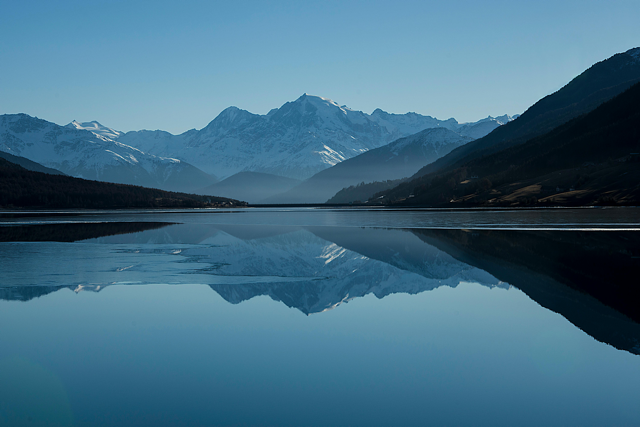
\includegraphics[width=.8\linewidth]{samplel.png}
		\caption{The caption of the figure.}
	\end{figure}	
	%% TODO: You can add the note here
	\note{}
\end{frame}

%% TODO: Uncomment the next four lines to enable this frame
% \begin{frame}{Methodology}
% 	%% TODO: You can add the note here
% 	\note{}
% \end{frame}

\begin{frame}[label=process1]{\texttt{Sample} Process 
  \hyperlink{algo1}{\beamerbutton{Algorithm}} 
  \hyperlink{pseudocode1}{\beamerbutton{Pseudocode}}
}
	\begin{columns}
		\column{0.3\textwidth}
		\centering
		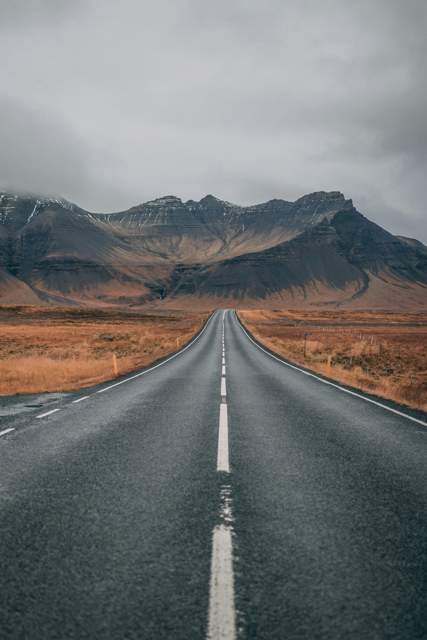
\includegraphics[height=1.8\textwidth]{samplev.png}
		\column{0.7\textwidth}
		\begin{itemize}
			\item \textbf{Goal:}
			\item \textbf{Result:}
			\item \textbf{Step:} 
			\item \textbf{Scope:}
		\end{itemize}
	\end{columns}
	%% TODO: You can add the note here
	\note{}
\end{frame}
								
\section{Result} 
			
\begin{frame}{Prototyping}
	%% TODO: Add your GitHub repository link here
	\textbf{GitHub repository:} \url{}
																
	%% TODO: Add your demo website link here
	\textbf{Demo Website:} \url{}
							
	\begin{columns}
		\column{0.5\textwidth}
		\begin{figure}
			\centering
			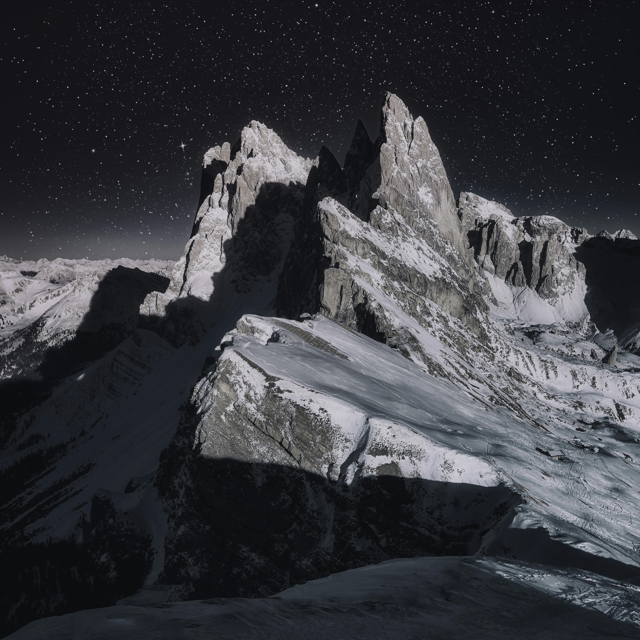
\includegraphics[width=.8\textwidth]{samples1.png}
			\caption{The caption of the figure.}
		\end{figure}	
		\column{0.5\textwidth}
		\begin{figure}
			\centering
			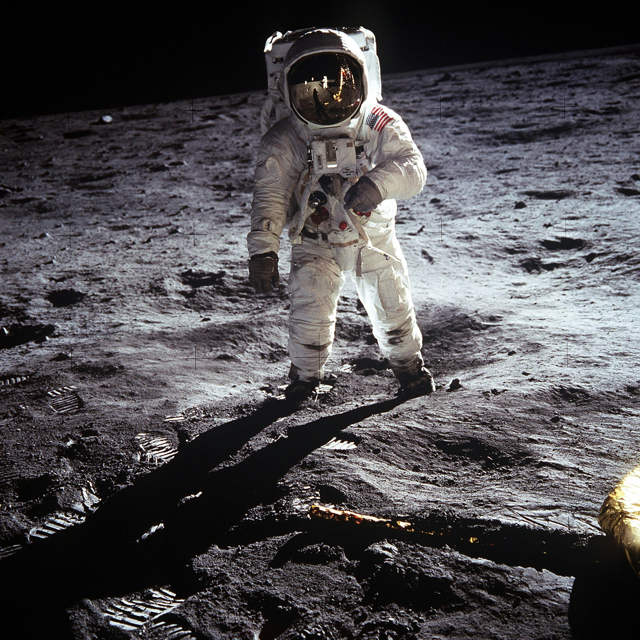
\includegraphics[width=.8\textwidth]{samples2.png}
			\caption{The caption of the figure.}
		\end{figure}
	\end{columns}
	%% TODO: You can add the note here
	\note{}
\end{frame}

%% TODO: Uncomment the next four lines to enable this frame
% \begin{frame}{Benchmark Results}
% 	%% TODO: You can add the note here
% 	\note{}	
% \end{frame}
			
\section{Discussion} 

%% TODO: Uncomment the next four lines to enable this frame
% \begin{frame}{Analysis}
% 	%% TODO: You can add the note here
% 	\note{}
% \end{frame}
	
\begin{frame}{Limitations}
	$\Rightarrow$ \textbf{Concluding statement.}
	%% TODO: You can add the note here
	\note{}
\end{frame}

\begin{frame}{Comparison}
	\begin{table}[ht]
		\centering
		\caption{Comparison of different methods (\protect\cmark: YES, \protect\xmark: NO).}
		%% Comment the next line if the table width is relatively small
		\resizebox{\textwidth}{!}{%
			\begin{tabular}{lcccccc}
				\hline
				          & \textbf{Your Method} & Method B & Method C & Method D & Method E & Method F \\ \hline
				Feature 1 & \cmark               & \cmark   & \xmark   & \cmark   & \xmark   & \cmark   \\ 
				Feature 2 & \cmark               & \xmark   & \cmark   & \cmark   & \cmark   & \xmark   \\ 
				Feature 3 & \xmark               & \cmark   & \cmark   & \xmark   & \xmark   & \cmark   \\ 
				Feature 4 & \cmark               & \cmark   & \xmark   & \xmark   & \cmark   & \xmark   \\ 
				Feature 5 & \xmark               & \xmark   & \cmark   & \cmark   & \xmark   & \cmark   \\ 
				Feature 6 & \cmark               & \xmark   & \cmark   & \xmark   & \xmark   & \xmark   \\ \hline
			\end{tabular}%
			%%TODO: Also comment this } to match the above command
		}
	\end{table}
	%% TODO: You can add the note here
	\note{}
\end{frame}
								 	
\section{Conclusion}

%% TODO: Uncomment the next four lines to enable this frame
% \begin{frame}{Summary}
% 	%% TODO: You can add the note here
% 	\note{}
% \end{frame}

%% TODO: Uncomment the next four lines to enable this frame
% \begin{frame}{Future works}		
% 	%% TODO: You can add the note here
% 	\note{}
% \end{frame}
			
\begin{frame}{Demonstration}
	\begin{block}{Process A}
	\end{block}
	\begin{block}{Scenario 1}
	\end{block}
	\begin{alertblock}{Scenario 2}
	\end{alertblock}
	\begin{block}{Process B}
	\end{block}
	%% TODO: You can add the note here
	\note{}
\end{frame}
											 			
%% Thank You frame
\begin{frame}
	\centering
	
\includegraphics[width=.7\linewidth]{thankyou}
	%% TODO: You can add the note here
	\note{}
\end{frame}
					
%% Appendix frames
\appendix
					
\begin{frame}[label=scope]{Scope \hyperlink{objectives}{\beamerbutton{Back to Objectives}}}
	%% TODO: You can add the note here
	\note{}
\end{frame}

\begin{frame}[label=algo1]{Formalizing - \texttt{Sample} Algorithm \hyperlink{process1}{\beamerbutton{Back to $\texttt{Sample}$ process}}}
	\begin{algorithm}[H]
		\small
		\caption{$(\text{Result}) \gets \texttt{Sample}(\text{Input1})$}
		\label{alg:algo1}
		\begin{algorithmic}[1]
			\Require $\text{Input1}$ is a predefined parameter.
			\State $\text{Set} \gets \emptyset$
			\For{$\text{element} \in \text{Input1}$}
			\If{$\text{Condition}(\text{element})$ is true}
			\State $\text{Set} \gets \text{Set} \cup \{\text{Process}(\text{element})\}$
			\Else
			\State \textbf{continue}
			\EndIf
			\EndFor
			\State $\text{Intermediate} \gets \texttt{Transform}(\text{Set})$
			\State \Return $\text{Result}$
		\end{algorithmic}
	\end{algorithm}
	%% TODO: You can add the note here
	\note{}
\end{frame}
	
\begin{frame}[label=pseudocode1]{Formalizing - \texttt{Sample} Pseudocode \hyperlink{process1}{\beamerbutton{Back to $\texttt{Sample}$ process}}}
	\begin{algorithm}[H]
		\small
		\caption{$(\text{Result}) \gets \texttt{Sample}(\text{Input1})$}
		\label{alg:pseudocode1}
		\begin{algorithmic}[1]
			\Require $\text{Input1}$ is a predefined parameter.
			\State $\text{Set} \gets \emptyset$
			\For{$\text{element} \in \text{Input1}$}
			\If{$\text{Condition}(\text{element})$ is true}
			\State $\text{Set} \gets \text{Set} \cup \{\text{Process}(\text{element})\}$
			\Else
			\State \textbf{continue}
			\EndIf
			\EndFor
			\State $\text{Intermediate} \gets \texttt{Transform}(\text{Set})$
			\State \Return $\text{Result}$
		\end{algorithmic}
	\end{algorithm}
	%% TODO: You can add the note here
	\note{}
\end{frame}

%% TODO: Uncomment the next four lines to enable this frame
% \begin{frame}{System architecture}
% 	%% TODO: You can add the note here
% 	\note{}
% \end{frame}

%% TODO: Uncomment the next four lines to enable this frame
% \begin{frame}{Tech strategy choices}
% 	%% TODO: You can add the note here
% 	\note{}
% \end{frame}

\begin{frame}[allowframebreaks, noframenumbering]{References}
	\printbibliography[heading=none]
\end{frame}
					
\end{document}